\documentclass[1p]{elsarticle_modified}
%\bibliographystyle{elsarticle-num}

%\usepackage[colorlinks]{hyperref}
%\usepackage{abbrmath_seonhwa} %\Abb, \Ascr, \Acal ,\Abf, \Afrak
\usepackage{amsfonts}
\usepackage{amssymb}
\usepackage{amsmath}
\usepackage{amsthm}
\usepackage{scalefnt}
\usepackage{amsbsy}
\usepackage{kotex}
\usepackage{caption}
\usepackage{subfig}
\usepackage{color}
\usepackage{graphicx}
\usepackage{xcolor} %% white, black, red, green, blue, cyan, magenta, yellow
\usepackage{float}
\usepackage{setspace}
\usepackage{hyperref}

\usepackage{tikz}
\usetikzlibrary{arrows}

\usepackage{multirow}
\usepackage{array} % fixed length table
\usepackage{hhline}

%%%%%%%%%%%%%%%%%%%%%
\makeatletter
\renewcommand*\env@matrix[1][\arraystretch]{%
	\edef\arraystretch{#1}%
	\hskip -\arraycolsep
	\let\@ifnextchar\new@ifnextchar
	\array{*\c@MaxMatrixCols c}}
\makeatother %https://tex.stackexchange.com/questions/14071/how-can-i-increase-the-line-spacing-in-a-matrix
%%%%%%%%%%%%%%%

\usepackage[normalem]{ulem}

\newcommand{\msout}[1]{\ifmmode\text{\sout{\ensuremath{#1}}}\else\sout{#1}\fi}
%SOURCE: \msout is \stkout macro in https://tex.stackexchange.com/questions/20609/strikeout-in-math-mode

\newcommand{\cancel}[1]{
	\ifmmode
	{\color{red}\msout{#1}}
	\else
	{\color{red}\sout{#1}}
	\fi
}

\newcommand{\add}[1]{
	{\color{blue}\uwave{#1}}
}

\newcommand{\replace}[2]{
	\ifmmode
	{\color{red}\msout{#1}}{\color{blue}\uwave{#2}}
	\else
	{\color{red}\sout{#1}}{\color{blue}\uwave{#2}}
	\fi
}

\newcommand{\Sol}{\mathcal{S}} %segment
\newcommand{\D}{D} %diagram
\newcommand{\A}{\mathcal{A}} %arc


%%%%%%%%%%%%%%%%%%%%%%%%%%%%%5 test

\def\sl{\operatorname{\textup{SL}}(2,\Cbb)}
\def\psl{\operatorname{\textup{PSL}}(2,\Cbb)}
\def\quan{\mkern 1mu \triangleright \mkern 1mu}

\theoremstyle{definition}
\newtheorem{thm}{Theorem}[section]
\newtheorem{prop}[thm]{Proposition}
\newtheorem{lem}[thm]{Lemma}
\newtheorem{ques}[thm]{Question}
\newtheorem{cor}[thm]{Corollary}
\newtheorem{defn}[thm]{Definition}
\newtheorem{exam}[thm]{Example}
\newtheorem{rmk}[thm]{Remark}
\newtheorem{alg}[thm]{Algorithm}

\newcommand{\I}{\sqrt{-1}}
\begin{document}

%\begin{frontmatter}
%
%\title{Boundary parabolic representations of knots up to 8 crossings}
%
%%% Group authors per affiliation:
%\author{Yunhi Cho} 
%\address{Department of Mathematics, University of Seoul, Seoul, Korea}
%\ead{yhcho@uos.ac.kr}
%
%
%\author{Seonhwa Kim} %\fnref{s_kim}}
%\address{Center for Geometry and Physics, Institute for Basic Science, Pohang, 37673, Korea}
%\ead{ryeona17@ibs.re.kr}
%
%\author{Hyuk Kim}
%\address{Department of Mathematical Sciences, Seoul National University, Seoul 08826, Korea}
%\ead{hyukkim@snu.ac.kr}
%
%\author{Seokbeom Yoon}
%\address{Department of Mathematical Sciences, Seoul National University, Seoul, 08826,  Korea}
%\ead{sbyoon15@snu.ac.kr}
%
%\begin{abstract}
%We find all boundary parabolic representation of knots up to 8 crossings.
%
%\end{abstract}
%\begin{keyword}
%    \MSC[2010] 57M25 
%\end{keyword}
%
%\end{frontmatter}

%\linenumbers
%\tableofcontents
%
\newcommand\colored[1]{\textcolor{white}{\rule[-0.35ex]{0.8em}{1.4ex}}\kern-0.8em\color{red} #1}%
%\newcommand\colored[1]{\textcolor{white}{ #1}\kern-2.17ex	\textcolor{white}{ #1}\kern-1.81ex	\textcolor{white}{ #1}\kern-2.15ex\color{red}#1	}

{\Large $\underline{12n_{0268}~(K12n_{0268})}$}

\setlength{\tabcolsep}{10pt}
\renewcommand{\arraystretch}{1.6}
\vspace{1cm}\begin{tabular}{m{100pt}>{\centering\arraybackslash}m{274pt}}
\multirow{5}{120pt}{
	\centering
	\includegraphics[width=112pt]{../../../GIT/diagram.site/Diagrams/png/2357_12n_0268.png}\\
\ \ \ A knot diagram\footnotemark}&
\allowdisplaybreaks
\textbf{Linearized knot diagam} \\
\cline{2-2}
 &
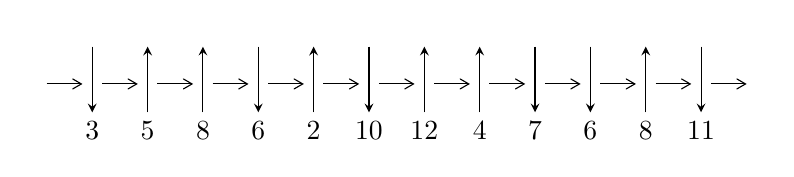
\begin{tikzpicture}[x=20pt, y=17pt]
	% nodes
	\node (C0) at (0, 0) {};
	\node (C1) at (1, 0) {};
	\node (C1U) at (1, +1) {};
	\node (C1D) at (1, -1) {3};

	\node (C2) at (2, 0) {};
	\node (C2U) at (2, +1) {};
	\node (C2D) at (2, -1) {5};

	\node (C3) at (3, 0) {};
	\node (C3U) at (3, +1) {};
	\node (C3D) at (3, -1) {8};

	\node (C4) at (4, 0) {};
	\node (C4U) at (4, +1) {};
	\node (C4D) at (4, -1) {6};

	\node (C5) at (5, 0) {};
	\node (C5U) at (5, +1) {};
	\node (C5D) at (5, -1) {2};

	\node (C6) at (6, 0) {};
	\node (C6U) at (6, +1) {};
	\node (C6D) at (6, -1) {10};

	\node (C7) at (7, 0) {};
	\node (C7U) at (7, +1) {};
	\node (C7D) at (7, -1) {12};

	\node (C8) at (8, 0) {};
	\node (C8U) at (8, +1) {};
	\node (C8D) at (8, -1) {4};

	\node (C9) at (9, 0) {};
	\node (C9U) at (9, +1) {};
	\node (C9D) at (9, -1) {7};

	\node (C10) at (10, 0) {};
	\node (C10U) at (10, +1) {};
	\node (C10D) at (10, -1) {6};

	\node (C11) at (11, 0) {};
	\node (C11U) at (11, +1) {};
	\node (C11D) at (11, -1) {8};

	\node (C12) at (12, 0) {};
	\node (C12U) at (12, +1) {};
	\node (C12D) at (12, -1) {11};
	\node (C13) at (13, 0) {};

	% arrows
	\draw[->,>={angle 60}]
	(C0) edge (C1) (C1) edge (C2) (C2) edge (C3) (C3) edge (C4) (C4) edge (C5) (C5) edge (C6) (C6) edge (C7) (C7) edge (C8) (C8) edge (C9) (C9) edge (C10) (C10) edge (C11) (C11) edge (C12) (C12) edge (C13) ;	\draw[->,>=stealth]
	(C1U) edge (C1D) (C2D) edge (C2U) (C3D) edge (C3U) (C4U) edge (C4D) (C5D) edge (C5U) (C6U) edge (C6D) (C7D) edge (C7U) (C8D) edge (C8U) (C9U) edge (C9D) (C10U) edge (C10D) (C11D) edge (C11U) (C12U) edge (C12D) ;
	\end{tikzpicture} \\
\hhline{~~} \\& 
\textbf{Solving Sequence} \\ \cline{2-2} 
 &
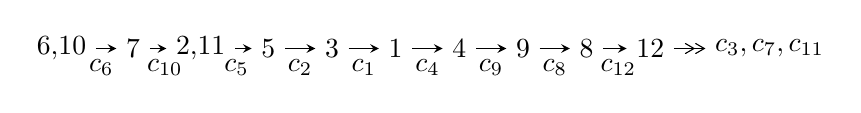
\begin{tikzpicture}[x=23pt, y=7pt]
	% node
	\node (A0) at (-1/8, 0) {6,10};
	\node (A1) at (1, 0) {7};
	\node (A2) at (33/16, 0) {2,11};
	\node (A3) at (25/8, 0) {5};
	\node (A4) at (33/8, 0) {3};
	\node (A5) at (41/8, 0) {1};
	\node (A6) at (49/8, 0) {4};
	\node (A7) at (57/8, 0) {9};
	\node (A8) at (65/8, 0) {8};
	\node (A9) at (73/8, 0) {12};
	\node (C1) at (1/2, -1) {$c_{6}$};
	\node (C2) at (3/2, -1) {$c_{10}$};
	\node (C3) at (21/8, -1) {$c_{5}$};
	\node (C4) at (29/8, -1) {$c_{2}$};
	\node (C5) at (37/8, -1) {$c_{1}$};
	\node (C6) at (45/8, -1) {$c_{4}$};
	\node (C7) at (53/8, -1) {$c_{9}$};
	\node (C8) at (61/8, -1) {$c_{8}$};
	\node (C9) at (69/8, -1) {$c_{12}$};
	\node (A10) at (11, 0) {$c_{3},c_{7},c_{11}$};

	% edge
	\draw[->,>=stealth]	
	(A0) edge (A1) (A1) edge (A2) (A2) edge (A3) (A3) edge (A4) (A4) edge (A5) (A5) edge (A6) (A6) edge (A7) (A7) edge (A8) (A8) edge (A9) ;
	\draw[->>,>={angle 60}]	
	(A9) edge (A10);
\end{tikzpicture} \\ 

\end{tabular} \\

\footnotetext{
The image of knot diagram is generated by the software ``\textbf{Draw programme}" developed by Andrew Bartholomew(\url{http://www.layer8.co.uk/maths/draw/index.htm\#Running-draw}), where we modified some parts for our purpose(\url{https://github.com/CATsTAILs/LinksPainter}).
}\phantom \\ \newline 
\centering \textbf{Ideals for irreducible components\footnotemark of $X_{\text{par}}$} 
 
\begin{align*}
I^u_{1}&=\langle 
-3.29204\times10^{20} u^{19}+9.27352\times10^{20} u^{18}+\cdots+2.43864\times10^{22} b-1.34033\times10^{22},\\
\phantom{I^u_{1}}&\phantom{= \langle  }-4.39429\times10^{21} u^{19}+1.24794\times10^{22} u^{18}+\cdots+9.75456\times10^{22} a-4.90353\times10^{23},\\
\phantom{I^u_{1}}&\phantom{= \langle  }u^{20}-3 u^{19}+\cdots+109 u+34\rangle \\
I^u_{2}&=\langle 
- u^2 a- u^2+b- a-1,\;2 u^3 a-4 u^2 a- u^3+4 a^2+6 a u-2 u^2+2 a- u+3,\;u^4- u^3+3 u^2-2 u+1\rangle \\
I^u_{3}&=\langle 
16 a^3 u+7 a^3-67 a^2 u+5 a^2+153 a u+61 b-36 a-158 u+91,\\
\phantom{I^u_{3}}&\phantom{= \langle  }a^4-3 a^3 u-5 a^3+14 a^2 u+9 a^2-26 a u-5 a+18 u-5,\;u^2+1\rangle \\
\\
\end{align*}
\raggedright * 3 irreducible components of $\dim_{\mathbb{C}}=0$, with total 36 representations.\\
\footnotetext{All coefficients of polynomials are rational numbers. But the coefficients are sometimes approximated in decimal forms when there is not enough margin.}
\newpage
\renewcommand{\arraystretch}{1}
\centering \section*{I. $I^u_{1}= \langle -3.29\times10^{20} u^{19}+9.27\times10^{20} u^{18}+\cdots+2.44\times10^{22} b-1.34\times10^{22},\;-4.39\times10^{21} u^{19}+1.25\times10^{22} u^{18}+\cdots+9.75\times10^{22} a-4.90\times10^{23},\;u^{20}-3 u^{19}+\cdots+109 u+34 \rangle$}
\flushleft \textbf{(i) Arc colorings}\\
\begin{tabular}{m{7pt} m{180pt} m{7pt} m{180pt} }
\flushright $a_{6}=$&$\begin{pmatrix}1\\0\end{pmatrix}$ \\
\flushright $a_{10}=$&$\begin{pmatrix}0\\u\end{pmatrix}$ \\
\flushright $a_{7}=$&$\begin{pmatrix}1\\u^2\end{pmatrix}$ \\
\flushright $a_{2}=$&$\begin{pmatrix}0.0450486 u^{19}-0.127934 u^{18}+\cdots+22.3785 u+5.02691\\0.0134995 u^{19}-0.0380274 u^{18}+\cdots+4.80738 u+0.549621\end{pmatrix}$ \\
\flushright $a_{11}=$&$\begin{pmatrix}- u\\u\end{pmatrix}$ \\
\flushright $a_{5}=$&$\begin{pmatrix}0.00528585 u^{19}-0.0271975 u^{18}+\cdots+10.3946 u-0.455911\\0.00385593 u^{19}-0.00521186 u^{18}+\cdots+2.81112 u-0.156325\end{pmatrix}$ \\
\flushright $a_{3}=$&$\begin{pmatrix}0.0193868 u^{19}-0.0630592 u^{18}+\cdots+16.0098 u+1.70343\\0.00436855 u^{19}-0.00558340 u^{18}+\cdots+4.17123 u+0.514711\end{pmatrix}$ \\
\flushright $a_{1}=$&$\begin{pmatrix}0.0197609 u^{19}-0.0588829 u^{18}+\cdots+10.4067 u+2.39866\\0.00436280 u^{19}-0.0129388 u^{18}+\cdots+2.70245 u+0.389051\end{pmatrix}$ \\
\flushright $a_{4}=$&$\begin{pmatrix}0.00914178 u^{19}-0.0324093 u^{18}+\cdots+13.2058 u-0.612236\\0.00385593 u^{19}-0.00521186 u^{18}+\cdots+2.81112 u-0.156325\end{pmatrix}$ \\
\flushright $a_{9}=$&$\begin{pmatrix}u\\u^3+u\end{pmatrix}$ \\
\flushright $a_{8}=$&$\begin{pmatrix}0.0119922 u^{19}-0.0407718 u^{18}+\cdots+4.81606 u-2.27540\\0.000306872 u^{19}-0.00141344 u^{18}+\cdots+0.273172 u-0.657170\end{pmatrix}$ \\
\flushright $a_{12}=$&$\begin{pmatrix}0.0193285 u^{19}-0.0576787 u^{18}+\cdots+9.52664 u+2.37998\\0.00479521 u^{19}-0.0141430 u^{18}+\cdots+3.58255 u+0.407734\end{pmatrix}$\\&\end{tabular}
\flushleft \textbf{(ii) Obstruction class $= -1$}\\~\\
\flushleft \textbf{(iii) Cusp Shapes $= -\frac{18686925740007476253183}{195091181117356896960512} u^{19}+\frac{11735621234030037886189}{48772795279339224240128} u^{18}+\cdots-\frac{9107616583783871001778045}{195091181117356896960512} u-\frac{82148572343533635819015}{5737975915216379322368}$}\\~\\
\newpage\renewcommand{\arraystretch}{1}
\flushleft \textbf{(iv) u-Polynomials at the component}\newline \\
\begin{tabular}{m{50pt}|m{274pt}}
Crossings & \hspace{64pt}u-Polynomials at each crossing \\
\hline $$\begin{aligned}c_{1},c_{4}\end{aligned}$$&$\begin{aligned}
&u^{20}+15 u^{19}+\cdots-353 u+16
\end{aligned}$\\
\hline $$\begin{aligned}c_{2},c_{5}\end{aligned}$$&$\begin{aligned}
&u^{20}+7 u^{19}+\cdots+35 u+4
\end{aligned}$\\
\hline $$\begin{aligned}c_{3},c_{8}\end{aligned}$$&$\begin{aligned}
&u^{20}- u^{19}+\cdots+2560 u+2048
\end{aligned}$\\
\hline $$\begin{aligned}c_{6},c_{9},c_{10}\end{aligned}$$&$\begin{aligned}
&u^{20}-3 u^{19}+\cdots+109 u+34
\end{aligned}$\\
\hline $$\begin{aligned}c_{7},c_{11}\end{aligned}$$&$\begin{aligned}
&u^{20}-3 u^{19}+\cdots-33 u+34
\end{aligned}$\\
\hline $$\begin{aligned}c_{12}\end{aligned}$$&$\begin{aligned}
&u^{20}+31 u^{19}+\cdots+32843 u+1156
\end{aligned}$\\
\hline
\end{tabular}\\~\\
\newpage\renewcommand{\arraystretch}{1}
\flushleft \textbf{(v) Riley Polynomials at the component}\newline \\
\begin{tabular}{m{50pt}|m{274pt}}
Crossings & \hspace{64pt}Riley Polynomials at each crossing \\
\hline $$\begin{aligned}c_{1},c_{4}\end{aligned}$$&$\begin{aligned}
&y^{20}-13 y^{19}+\cdots-93409 y+256
\end{aligned}$\\
\hline $$\begin{aligned}c_{2},c_{5}\end{aligned}$$&$\begin{aligned}
&y^{20}+15 y^{19}+\cdots-353 y+16
\end{aligned}$\\
\hline $$\begin{aligned}c_{3},c_{8}\end{aligned}$$&$\begin{aligned}
&y^{20}+71 y^{19}+\cdots+13893632 y+4194304
\end{aligned}$\\
\hline $$\begin{aligned}c_{6},c_{9},c_{10}\end{aligned}$$&$\begin{aligned}
&y^{20}+3 y^{19}+\cdots+30619 y+1156
\end{aligned}$\\
\hline $$\begin{aligned}c_{7},c_{11}\end{aligned}$$&$\begin{aligned}
&y^{20}+31 y^{19}+\cdots+32843 y+1156
\end{aligned}$\\
\hline $$\begin{aligned}c_{12}\end{aligned}$$&$\begin{aligned}
&y^{20}-73 y^{19}+\cdots-208085985 y+1336336
\end{aligned}$\\
\hline
\end{tabular}\\~\\
\newpage\flushleft \textbf{(vi) Complex Volumes and Cusp Shapes}
$$\begin{array}{c|c|c}  
\text{Solutions to }I^u_{1}& \I (\text{vol} + \sqrt{-1}CS) & \text{Cusp shape}\\
 \hline 
\begin{aligned}
u &= -0.016951 + 0.789231 I \\
a &= -0.147460 - 1.134770 I \\
b &= \phantom{-}0.508184 + 0.603985 I\end{aligned}
 & \phantom{-}1.11325 + 1.38275 I & \phantom{-}7.09119 - 4.02054 I \\ \hline\begin{aligned}
u &= -0.016951 - 0.789231 I \\
a &= -0.147460 + 1.134770 I \\
b &= \phantom{-}0.508184 - 0.603985 I\end{aligned}
 & \phantom{-}1.11325 - 1.38275 I & \phantom{-}7.09119 + 4.02054 I \\ \hline\begin{aligned}
u &= -0.409805 + 0.654210 I \\
a &= \phantom{-}0.913159 - 0.159905 I \\
b &= -0.266779 + 0.021705 I\end{aligned}
 & \phantom{-}0.11722 + 1.46637 I & \phantom{-}1.49691 - 4.73539 I \\ \hline\begin{aligned}
u &= -0.409805 - 0.654210 I \\
a &= \phantom{-}0.913159 + 0.159905 I \\
b &= -0.266779 - 0.021705 I\end{aligned}
 & \phantom{-}0.11722 - 1.46637 I & \phantom{-}1.49691 + 4.73539 I \\ \hline\begin{aligned}
u &= \phantom{-}0.154412 + 0.621344 I \\
a &= -1.91384 - 1.58582 I \\
b &= \phantom{-}0.530147 - 0.944937 I\end{aligned}
 & \phantom{-}0.12177 - 2.86051 I & \phantom{-}4.18275 - 0.60909 I \\ \hline\begin{aligned}
u &= \phantom{-}0.154412 - 0.621344 I \\
a &= -1.91384 + 1.58582 I \\
b &= \phantom{-}0.530147 + 0.944937 I\end{aligned}
 & \phantom{-}0.12177 + 2.86051 I & \phantom{-}4.18275 + 0.60909 I \\ \hline\begin{aligned}
u &= -0.18250 + 1.41448 I \\
a &= \phantom{-}1.66337 + 0.44996 I \\
b &= -0.729471 - 0.781970 I\end{aligned}
 & \phantom{-}7.73611 + 5.17350 I & \phantom{-}7.90966 - 4.84500 I \\ \hline\begin{aligned}
u &= -0.18250 - 1.41448 I \\
a &= \phantom{-}1.66337 - 0.44996 I \\
b &= -0.729471 + 0.781970 I\end{aligned}
 & \phantom{-}7.73611 - 5.17350 I & \phantom{-}7.90966 + 4.84500 I \\ \hline\begin{aligned}
u &= -0.120113 + 0.255851 I \\
a &= \phantom{-}2.56623 + 3.01463 I \\
b &= \phantom{-}0.203906 + 0.753665 I\end{aligned}
 & -1.66738 + 1.58596 I & -6.75642 - 4.62170 I \\ \hline\begin{aligned}
u &= -0.120113 - 0.255851 I \\
a &= \phantom{-}2.56623 - 3.01463 I \\
b &= \phantom{-}0.203906 - 0.753665 I\end{aligned}
 & -1.66738 - 1.58596 I & -6.75642 + 4.62170 I\\
 \hline 
 \end{array}$$\newpage$$\begin{array}{c|c|c}  
\text{Solutions to }I^u_{1}& \I (\text{vol} + \sqrt{-1}CS) & \text{Cusp shape}\\
 \hline 
\begin{aligned}
u &= -0.57886 + 1.65257 I \\
a &= \phantom{-}1.15768 - 1.00754 I \\
b &= -0.73327 + 1.21762 I\end{aligned}
 & \phantom{-}6.46005 - 0.37754 I & \phantom{-}1.69270 + 0.75958 I \\ \hline\begin{aligned}
u &= -0.57886 - 1.65257 I \\
a &= \phantom{-}1.15768 + 1.00754 I \\
b &= -0.73327 - 1.21762 I\end{aligned}
 & \phantom{-}6.46005 + 0.37754 I & \phantom{-}1.69270 - 0.75958 I \\ \hline\begin{aligned}
u &= \phantom{-}0.83952 + 1.68636 I \\
a &= \phantom{-}1.91623 - 0.59074 I \\
b &= -0.80508 + 1.30894 I\end{aligned}
 & -13.2323 - 12.8519 I & \phantom{-}1.25558 + 5.23566 I \\ \hline\begin{aligned}
u &= \phantom{-}0.83952 - 1.68636 I \\
a &= \phantom{-}1.91623 + 0.59074 I \\
b &= -0.80508 - 1.30894 I\end{aligned}
 & -13.2323 + 12.8519 I & \phantom{-}1.25558 - 5.23566 I \\ \hline\begin{aligned}
u &= \phantom{-}1.22594 + 1.55065 I \\
a &= \phantom{-}1.69696 + 0.72298 I \\
b &= -1.37246 - 0.39498 I\end{aligned}
 & -10.36440 - 5.35439 I & \phantom{-}2.02942 + 1.66531 I \\ \hline\begin{aligned}
u &= \phantom{-}1.22594 - 1.55065 I \\
a &= \phantom{-}1.69696 - 0.72298 I \\
b &= -1.37246 + 0.39498 I\end{aligned}
 & -10.36440 + 5.35439 I & \phantom{-}2.02942 - 1.66531 I \\ \hline\begin{aligned}
u &= -1.85145 + 1.14515 I \\
a &= \phantom{-}0.648918 + 0.734717 I \\
b &= -0.25500 - 1.69562 I\end{aligned}
 & -5.65348 + 3.36046 I & \phantom{-}0.05819 - 1.65611 I \\ \hline\begin{aligned}
u &= -1.85145 - 1.14515 I \\
a &= \phantom{-}0.648918 - 0.734717 I \\
b &= -0.25500 + 1.69562 I\end{aligned}
 & -5.65348 - 3.36046 I & \phantom{-}0.05819 + 1.65611 I \\ \hline\begin{aligned}
u &= \phantom{-}2.43981 + 0.93238 I \\
a &= \phantom{-}0.616388 + 1.146420 I \\
b &= -0.58018 - 1.86831 I\end{aligned}
 & -17.5295 + 2.0815 I & \phantom{-0.000000 }      -6
0. 10   - 0.732251 I \\ \hline\begin{aligned}
u &= \phantom{-}2.43981 - 0.93238 I \\
a &= \phantom{-}0.616388 - 1.146420 I \\
b &= -0.58018 + 1.86831 I\end{aligned}
 & -17.5295 - 2.0815 I & \phantom{-0.000000 -}     -6
0. 10   + 0.732251 I\\
 \hline 
 \end{array}$$\newpage\newpage\renewcommand{\arraystretch}{1}
\centering \section*{II. $I^u_{2}= \langle - u^2 a- u^2+b- a-1,\;2 u^3 a- u^3+\cdots+2 a+3,\;u^4- u^3+3 u^2-2 u+1 \rangle$}
\flushleft \textbf{(i) Arc colorings}\\
\begin{tabular}{m{7pt} m{180pt} m{7pt} m{180pt} }
\flushright $a_{6}=$&$\begin{pmatrix}1\\0\end{pmatrix}$ \\
\flushright $a_{10}=$&$\begin{pmatrix}0\\u\end{pmatrix}$ \\
\flushright $a_{7}=$&$\begin{pmatrix}1\\u^2\end{pmatrix}$ \\
\flushright $a_{2}=$&$\begin{pmatrix}a\\u^2 a+u^2+a+1\end{pmatrix}$ \\
\flushright $a_{11}=$&$\begin{pmatrix}- u\\u\end{pmatrix}$ \\
\flushright $a_{5}=$&$\begin{pmatrix}- u^2 a+\frac{1}{2} u^3-2 u^2+\frac{3}{2} u-\frac{1}{2}\\u^2 a+u^2+a\end{pmatrix}$ \\
\flushright $a_{3}=$&$\begin{pmatrix}\frac{1}{2} u^3- u^2+a+\frac{3}{2} u-\frac{1}{2}\\u^2 a+u^2+a\end{pmatrix}$ \\
\flushright $a_{1}=$&$\begin{pmatrix}-1\\0\end{pmatrix}$ \\
\flushright $a_{4}=$&$\begin{pmatrix}\frac{1}{2} u^3- u^2+a+\frac{3}{2} u-\frac{1}{2}\\u^2 a+u^2+a\end{pmatrix}$ \\
\flushright $a_{9}=$&$\begin{pmatrix}u\\u^3+u\end{pmatrix}$ \\
\flushright $a_{8}=$&$\begin{pmatrix}u\\u^3+u\end{pmatrix}$ \\
\flushright $a_{12}=$&$\begin{pmatrix}- u^2-1\\u^2\end{pmatrix}$\\&\end{tabular}
\flushleft \textbf{(ii) Obstruction class $= 1$}\\~\\
\flushleft \textbf{(iii) Cusp Shapes $= -\frac{7}{2} u^3 a- u^2 a-\frac{1}{2} u^3-\frac{11}{2} a u-3 u^2-\frac{7}{2} a+\frac{11}{2} u-\frac{11}{2}$}\\~\\
\newpage\renewcommand{\arraystretch}{1}
\flushleft \textbf{(iv) u-Polynomials at the component}\newline \\
\begin{tabular}{m{50pt}|m{274pt}}
Crossings & \hspace{64pt}u-Polynomials at each crossing \\
\hline $$\begin{aligned}c_{1},c_{4},c_{5}\end{aligned}$$&$\begin{aligned}
&(u^2- u+1)^4
\end{aligned}$\\
\hline $$\begin{aligned}c_{2}\end{aligned}$$&$\begin{aligned}
&(u^2+u+1)^4
\end{aligned}$\\
\hline $$\begin{aligned}c_{3},c_{8}\end{aligned}$$&$\begin{aligned}
&u^8
\end{aligned}$\\
\hline $$\begin{aligned}c_{6}\end{aligned}$$&$\begin{aligned}
&(u^4- u^3+3 u^2-2 u+1)^2
\end{aligned}$\\
\hline $$\begin{aligned}c_{7}\end{aligned}$$&$\begin{aligned}
&(u^4- u^3+u^2+1)^2
\end{aligned}$\\
\hline $$\begin{aligned}c_{9},c_{10},c_{12}\end{aligned}$$&$\begin{aligned}
&(u^4+u^3+3 u^2+2 u+1)^2
\end{aligned}$\\
\hline $$\begin{aligned}c_{11}\end{aligned}$$&$\begin{aligned}
&(u^4+u^3+u^2+1)^2
\end{aligned}$\\
\hline
\end{tabular}\\~\\
\newpage\renewcommand{\arraystretch}{1}
\flushleft \textbf{(v) Riley Polynomials at the component}\newline \\
\begin{tabular}{m{50pt}|m{274pt}}
Crossings & \hspace{64pt}Riley Polynomials at each crossing \\
\hline $$\begin{aligned}c_{1},c_{2},c_{4}\\c_{5}\end{aligned}$$&$\begin{aligned}
&(y^2+y+1)^4
\end{aligned}$\\
\hline $$\begin{aligned}c_{3},c_{8}\end{aligned}$$&$\begin{aligned}
&y^8
\end{aligned}$\\
\hline $$\begin{aligned}c_{6},c_{9},c_{10}\\c_{12}\end{aligned}$$&$\begin{aligned}
&(y^4+5 y^3+7 y^2+2 y+1)^2
\end{aligned}$\\
\hline $$\begin{aligned}c_{7},c_{11}\end{aligned}$$&$\begin{aligned}
&(y^4+y^3+3 y^2+2 y+1)^2
\end{aligned}$\\
\hline
\end{tabular}\\~\\
\newpage\flushleft \textbf{(vi) Complex Volumes and Cusp Shapes}
$$\begin{array}{c|c|c}  
\text{Solutions to }I^u_{2}& \I (\text{vol} + \sqrt{-1}CS) & \text{Cusp shape}\\
 \hline 
\begin{aligned}
u &= \phantom{-}0.395123 + 0.506844 I \\
a &= -0.893973 - 1.010300 I \\
b &= \phantom{-}0.500000 - 0.866025 I\end{aligned}
 & -0.21101 - 3.44499 I & -2.28131 + 9.48913 I \\ \hline\begin{aligned}
u &= \phantom{-}0.395123 + 0.506844 I \\
a &= -0.178069 + 0.596972 I \\
b &= \phantom{-}0.500000 + 0.866025 I\end{aligned}
 & -0.211005 + 0.614778 I & \phantom{-}0.065036 - 0.652246 I \\ \hline\begin{aligned}
u &= \phantom{-}0.395123 - 0.506844 I \\
a &= -0.893973 + 1.010300 I \\
b &= \phantom{-}0.500000 + 0.866025 I\end{aligned}
 & -0.21101 + 3.44499 I & -2.28131 - 9.48913 I \\ \hline\begin{aligned}
u &= \phantom{-}0.395123 - 0.506844 I \\
a &= -0.178069 - 0.596972 I \\
b &= \phantom{-}0.500000 - 0.866025 I\end{aligned}
 & -0.211005 - 0.614778 I & \phantom{-}0.065036 + 0.652246 I \\ \hline\begin{aligned}
u &= \phantom{-}0.10488 + 1.55249 I \\
a &= -1.202340 - 0.666019 I \\
b &= \phantom{-}0.500000 + 0.866025 I\end{aligned}
 & \phantom{-}6.79074 - 1.13408 I & \phantom{-}4.18309 + 3.88645 I \\ \hline\begin{aligned}
u &= \phantom{-}0.10488 + 1.55249 I \\
a &= -1.47562 + 0.50824 I \\
b &= \phantom{-}0.500000 - 0.866025 I\end{aligned}
 & \phantom{-}6.79074 - 5.19385 I & -0.84181 + 3.92087 I \\ \hline\begin{aligned}
u &= \phantom{-}0.10488 - 1.55249 I \\
a &= -1.202340 + 0.666019 I \\
b &= \phantom{-}0.500000 - 0.866025 I\end{aligned}
 & \phantom{-}6.79074 + 1.13408 I & \phantom{-}4.18309 - 3.88645 I \\ \hline\begin{aligned}
u &= \phantom{-}0.10488 - 1.55249 I \\
a &= -1.47562 - 0.50824 I \\
b &= \phantom{-}0.500000 + 0.866025 I\end{aligned}
 & \phantom{-}6.79074 + 5.19385 I & -0.84181 - 3.92087 I\\
 \hline 
 \end{array}$$\newpage\newpage\renewcommand{\arraystretch}{1}
\centering \section*{III. $I^u_{3}= \langle 16 a^3 u-67 a^2 u+\cdots-36 a+91,\;-3 a^3 u+14 a^2 u+\cdots-5 a-5,\;u^2+1 \rangle$}
\flushleft \textbf{(i) Arc colorings}\\
\begin{tabular}{m{7pt} m{180pt} m{7pt} m{180pt} }
\flushright $a_{6}=$&$\begin{pmatrix}1\\0\end{pmatrix}$ \\
\flushright $a_{10}=$&$\begin{pmatrix}0\\u\end{pmatrix}$ \\
\flushright $a_{7}=$&$\begin{pmatrix}1\\-1\end{pmatrix}$ \\
\flushright $a_{2}=$&$\begin{pmatrix}a\\-0.262295 a^{3} u+1.09836 a^{2} u+\cdots+0.590164 a-1.49180\end{pmatrix}$ \\
\flushright $a_{11}=$&$\begin{pmatrix}- u\\u\end{pmatrix}$ \\
\flushright $a_{5}=$&$\begin{pmatrix}-0.557377 a^{3} u+1.45902 a^{2} u+\cdots+4.75410 a-4.29508\\0.0983607 a^{3} u+0.213115 a^{2} u+\cdots-0.721311 a-0.0655738\end{pmatrix}$ \\
\flushright $a_{3}=$&$\begin{pmatrix}0.196721 a^{3} u+0.426230 a^{2} u+\cdots-1.44262 a-0.131148\\-0.475410 a^{3} u+0.803279 a^{2} u+\cdots+3.81967 a-3.01639\end{pmatrix}$ \\
\flushright $a_{1}=$&$\begin{pmatrix}0.114754 a^{3} u+0.0819672 a^{2} u+\cdots-2.50820 a+0.590164\\-0.114754 a^{3} u-0.0819672 a^{2} u+\cdots+2.50820 a-0.590164\end{pmatrix}$ \\
\flushright $a_{4}=$&$\begin{pmatrix}-0.459016 a^{3} u+1.67213 a^{2} u+\cdots+4.03279 a-4.36066\\0.0983607 a^{3} u+0.213115 a^{2} u+\cdots-0.721311 a-0.0655738\end{pmatrix}$ \\
\flushright $a_{9}=$&$\begin{pmatrix}u\\0\end{pmatrix}$ \\
\flushright $a_{8}=$&$\begin{pmatrix}0.262295 a^{3} u-1.09836 a^{2} u+\cdots-1.59016 a+3.49180\\-0.262295 a^{3} u+1.09836 a^{2} u+\cdots+1.59016 a-2.49180\end{pmatrix}$ \\
\flushright $a_{12}=$&$\begin{pmatrix}0.114754 a^{3} u+0.0819672 a^{2} u+\cdots-2.50820 a+0.590164\\-0.114754 a^{3} u-0.0819672 a^{2} u+\cdots+2.50820 a-0.590164\end{pmatrix}$\\&\end{tabular}
\flushleft \textbf{(ii) Obstruction class $= 1$}\\~\\
\flushleft \textbf{(iii) Cusp Shapes $= \frac{40}{61} a^3 u+\frac{48}{61} a^3-\frac{320}{61} a^2 u-\frac{140}{61} a^2+\frac{840}{61} a u+\frac{32}{61} a-\frac{944}{61} u+\frac{380}{61}$}\\~\\
\newpage\renewcommand{\arraystretch}{1}
\flushleft \textbf{(iv) u-Polynomials at the component}\newline \\
\begin{tabular}{m{50pt}|m{274pt}}
Crossings & \hspace{64pt}u-Polynomials at each crossing \\
\hline $$\begin{aligned}c_{1},c_{4}\end{aligned}$$&$\begin{aligned}
&(u^4- u^3+3 u^2-2 u+1)^2
\end{aligned}$\\
\hline $$\begin{aligned}c_{2}\end{aligned}$$&$\begin{aligned}
&(u^4- u^3+u^2+1)^2
\end{aligned}$\\
\hline $$\begin{aligned}c_{3},c_{8}\end{aligned}$$&$\begin{aligned}
&u^8-5 u^6+7 u^4-2 u^2+1
\end{aligned}$\\
\hline $$\begin{aligned}c_{5}\end{aligned}$$&$\begin{aligned}
&(u^4+u^3+u^2+1)^2
\end{aligned}$\\
\hline $$\begin{aligned}c_{6},c_{7},c_{9}\\c_{10},c_{11}\end{aligned}$$&$\begin{aligned}
&(u^2+1)^4
\end{aligned}$\\
\hline $$\begin{aligned}c_{12}\end{aligned}$$&$\begin{aligned}
&(u+1)^8
\end{aligned}$\\
\hline
\end{tabular}\\~\\
\newpage\renewcommand{\arraystretch}{1}
\flushleft \textbf{(v) Riley Polynomials at the component}\newline \\
\begin{tabular}{m{50pt}|m{274pt}}
Crossings & \hspace{64pt}Riley Polynomials at each crossing \\
\hline $$\begin{aligned}c_{1},c_{4}\end{aligned}$$&$\begin{aligned}
&(y^4+5 y^3+7 y^2+2 y+1)^2
\end{aligned}$\\
\hline $$\begin{aligned}c_{2},c_{5}\end{aligned}$$&$\begin{aligned}
&(y^4+y^3+3 y^2+2 y+1)^2
\end{aligned}$\\
\hline $$\begin{aligned}c_{3},c_{8}\end{aligned}$$&$\begin{aligned}
&(y^4-5 y^3+7 y^2-2 y+1)^2
\end{aligned}$\\
\hline $$\begin{aligned}c_{6},c_{7},c_{9}\\c_{10},c_{11}\end{aligned}$$&$\begin{aligned}
&(y+1)^8
\end{aligned}$\\
\hline $$\begin{aligned}c_{12}\end{aligned}$$&$\begin{aligned}
&(y-1)^8
\end{aligned}$\\
\hline
\end{tabular}\\~\\
\newpage\flushleft \textbf{(vi) Complex Volumes and Cusp Shapes}
$$\begin{array}{c|c|c}  
\text{Solutions to }I^u_{3}& \I (\text{vol} + \sqrt{-1}CS) & \text{Cusp shape}\\
 \hline 
\begin{aligned}
u &= \phantom{-0.000000 -}1.000000 I \\
a &= \phantom{-}1.04872 + 1.17889 I \\
b &= \phantom{-}0.351808 + 0.720342 I\end{aligned}
 & -0.21101 + 1.41510 I & \phantom{-}0.17326 - 4.90874 I \\ \hline\begin{aligned}
u &= \phantom{-0.000000 -}1.000000 I \\
a &= \phantom{-}1.52617 - 1.31052 I \\
b &= -0.851808 + 0.911292 I\end{aligned}
 & \phantom{-}6.79074 - 3.16396 I & \phantom{-}3.82674 + 2.56480 I \\ \hline\begin{aligned}
u &= \phantom{-0.000000 -}1.000000 I \\
a &= \phantom{-}2.17745 + 0.51206 I \\
b &= -0.851808 - 0.911292 I\end{aligned}
 & \phantom{-}6.79074 + 3.16396 I & \phantom{-}3.82674 - 2.56480 I \\ \hline\begin{aligned}
u &= \phantom{-0.000000 -}1.000000 I \\
a &= \phantom{-}0.24766 + 2.61957 I \\
b &= \phantom{-}0.351808 - 0.720342 I\end{aligned}
 & -0.21101 - 1.41510 I & \phantom{-}0.17326 + 4.90874 I \\ \hline\begin{aligned}
u &= \phantom{-0.000000 } -1.000000 I \\
a &= \phantom{-}1.04872 - 1.17889 I \\
b &= \phantom{-}0.351808 - 0.720342 I\end{aligned}
 & -0.21101 - 1.41510 I & \phantom{-}0.17326 + 4.90874 I \\ \hline\begin{aligned}
u &= \phantom{-0.000000 } -1.000000 I \\
a &= \phantom{-}1.52617 + 1.31052 I \\
b &= -0.851808 - 0.911292 I\end{aligned}
 & \phantom{-}6.79074 + 3.16396 I & \phantom{-}3.82674 - 2.56480 I \\ \hline\begin{aligned}
u &= \phantom{-0.000000 } -1.000000 I \\
a &= \phantom{-}2.17745 - 0.51206 I \\
b &= -0.851808 + 0.911292 I\end{aligned}
 & \phantom{-}6.79074 - 3.16396 I & \phantom{-}3.82674 + 2.56480 I \\ \hline\begin{aligned}
u &= \phantom{-0.000000 } -1.000000 I \\
a &= \phantom{-}0.24766 - 2.61957 I \\
b &= \phantom{-}0.351808 + 0.720342 I\end{aligned}
 & -0.21101 + 1.41510 I & \phantom{-}0.17326 - 4.90874 I\\
 \hline 
 \end{array}$$\newpage
\newpage\renewcommand{\arraystretch}{1}
\centering \section*{ IV. u-Polynomials}
\begin{tabular}{m{50pt}|m{274pt}}
Crossings & \hspace{64pt}u-Polynomials at each crossing \\
\hline $$\begin{aligned}c_{1},c_{4}\end{aligned}$$&$\begin{aligned}
&(u^2- u+1)^4(u^4- u^3+3 u^2-2 u+1)^2\\
&\cdot(u^{20}+15 u^{19}+\cdots-353 u+16)
\end{aligned}$\\
\hline $$\begin{aligned}c_{2}\end{aligned}$$&$\begin{aligned}
&((u^2+u+1)^4)(u^4- u^3+u^2+1)^2(u^{20}+7 u^{19}+\cdots+35 u+4)
\end{aligned}$\\
\hline $$\begin{aligned}c_{3},c_{8}\end{aligned}$$&$\begin{aligned}
&u^8(u^8-5 u^6+\cdots-2 u^2+1)(u^{20}-u^{19}+\cdots+2560 u+2048)
\end{aligned}$\\
\hline $$\begin{aligned}c_{5}\end{aligned}$$&$\begin{aligned}
&((u^2- u+1)^4)(u^4+u^3+u^2+1)^2(u^{20}+7 u^{19}+\cdots+35 u+4)
\end{aligned}$\\
\hline $$\begin{aligned}c_{6}\end{aligned}$$&$\begin{aligned}
&((u^2+1)^4)(u^4- u^3+3 u^2-2 u+1)^{2}(u^{20}-3 u^{19}+\cdots+109 u+34)
\end{aligned}$\\
\hline $$\begin{aligned}c_{7}\end{aligned}$$&$\begin{aligned}
&((u^2+1)^4)(u^4- u^3+u^2+1)^2(u^{20}-3 u^{19}+\cdots-33 u+34)
\end{aligned}$\\
\hline $$\begin{aligned}c_{9},c_{10}\end{aligned}$$&$\begin{aligned}
&((u^2+1)^4)(u^4+u^3+3 u^2+2 u+1)^{2}(u^{20}-3 u^{19}+\cdots+109 u+34)
\end{aligned}$\\
\hline $$\begin{aligned}c_{11}\end{aligned}$$&$\begin{aligned}
&((u^2+1)^4)(u^4+u^3+u^2+1)^2(u^{20}-3 u^{19}+\cdots-33 u+34)
\end{aligned}$\\
\hline $$\begin{aligned}c_{12}\end{aligned}$$&$\begin{aligned}
&(u+1)^8(u^4+u^3+3 u^2+2 u+1)^2\\
&\cdot(u^{20}+31 u^{19}+\cdots+32843 u+1156)
\end{aligned}$\\
\hline
\end{tabular}\newpage\renewcommand{\arraystretch}{1}
\centering \section*{ V. Riley Polynomials}
\begin{tabular}{m{50pt}|m{274pt}}
Crossings & \hspace{64pt}Riley Polynomials at each crossing \\
\hline $$\begin{aligned}c_{1},c_{4}\end{aligned}$$&$\begin{aligned}
&(y^2+y+1)^4(y^4+5 y^3+7 y^2+2 y+1)^2\\
&\cdot(y^{20}-13 y^{19}+\cdots-93409 y+256)
\end{aligned}$\\
\hline $$\begin{aligned}c_{2},c_{5}\end{aligned}$$&$\begin{aligned}
&(y^2+y+1)^4(y^4+y^3+3 y^2+2 y+1)^2\\
&\cdot(y^{20}+15 y^{19}+\cdots-353 y+16)
\end{aligned}$\\
\hline $$\begin{aligned}c_{3},c_{8}\end{aligned}$$&$\begin{aligned}
&y^8(y^4-5 y^3+7 y^2-2 y+1)^2\\
&\cdot(y^{20}+71 y^{19}+\cdots+13893632 y+4194304)
\end{aligned}$\\
\hline $$\begin{aligned}c_{6},c_{9},c_{10}\end{aligned}$$&$\begin{aligned}
&(y+1)^8(y^4+5 y^3+7 y^2+2 y+1)^2\\
&\cdot(y^{20}+3 y^{19}+\cdots+30619 y+1156)
\end{aligned}$\\
\hline $$\begin{aligned}c_{7},c_{11}\end{aligned}$$&$\begin{aligned}
&(y+1)^8(y^4+y^3+3 y^2+2 y+1)^2\\
&\cdot(y^{20}+31 y^{19}+\cdots+32843 y+1156)
\end{aligned}$\\
\hline $$\begin{aligned}c_{12}\end{aligned}$$&$\begin{aligned}
&(y-1)^8(y^4+5 y^3+7 y^2+2 y+1)^2\\
&\cdot(y^{20}-73 y^{19}+\cdots-208085985 y+1336336)
\end{aligned}$\\
\hline
\end{tabular}
\vskip 2pc
\end{document}